\documentclass[a4paper,12pt]{article}

% 导言区
\usepackage{titlesec}
\usepackage{lipsum} % 示例用,可以删除
\usepackage{geometry}
\usepackage{setspace}
\usepackage{amsmath} % 用于数学公式
\usepackage{graphicx} % 用于插入图片
\usepackage{float}
\usepackage{lipsum} % 用于生成虚拟文本
\usepackage{ctex} % 导入 ctex 包以支持中文
\usepackage{xeCJK}
\usepackage{titlesec} % 导入 titlesec 包以定制标题样式
\usepackage{fontspec} % 用于设置中文字体
\usepackage{amsfonts}
\usepackage{amsmath} % 提供 \text 和 \tanh 命令
\usepackage{bm}      % 提供 \bm 命令用于粗体

% 目录设置
\usepackage[nottoc,notlot,notlof]{tocbibind}
\usepackage{enumitem}
% 页面设置
\geometry{margin=1in}

% 标题设置
\titleformat{\section}{\normalfont\Large\bfseries}{\thesection}{1em}{}
\titleformat{\subsection}{\normalfont\large\bfseries}{\thesubsection}{1em}{}
\titleformat{\subsubsection}{\normalfont\normalsize\bfseries}{\thesubsubsection}{1em}{}

% 行间距设置
\onehalfspacing

% 文档信息
\title{商业模式设计}
\author{需求不寄小分队}
\date{\today}

\begin{document}

    \maketitle

% 添加目录
    \tableofcontents

    \section{团队成员}
    \begin{itemize}
        \item 211250124 程智镝
        \item 211250122 刘辉
        \item 211250159 陈凌
        \item 211250158 李忠信
    \end{itemize}

    \subsection{度量数值}

    \section{文档简介}
    我们按照商业模式画布,使用教材讲述的六种设计方法,对之前的分析进行了梳理与完善。较之之前的
    分析结果,更加清楚地完善了产品的价值追求。明确了我们产品的创意方向,与较之其他产品的关键性
    创意。摒弃了之前一些大而空的产品构思,分析结果更加具体,明确。

    \section{客户洞察}
    \subsection{高校教师}
    作为一款大众会议虚拟软件,我们意识到在疫情过后,学校师生对会议软件的需求量大幅增加。因此,我们希望打造一个专门服务于教学领域的教育软件。除了提供基本的会议功能外,我们还致力于为教师和学生提供更专业、更便捷的服务,例如在线答题、定期会议、讨论小组等功能,以模拟线下教学的模式。我们的目标是让教师和学生在使用我们的软件时能够体验到线下教学的特色,同时享受线上会议的高效便捷,从而实现教学的智能化与便利化。

    下图展示了一个高校老师小陈由于疫情原因无法线下上课,教学问题成为他急需解决的问题。我们希望通过我们的软件,能够帮助像小陈老师这样的教师解决线上教学所面临的挑战,提升他们的教学效率和质量。
    \begin{figure}[h]
        \centering
        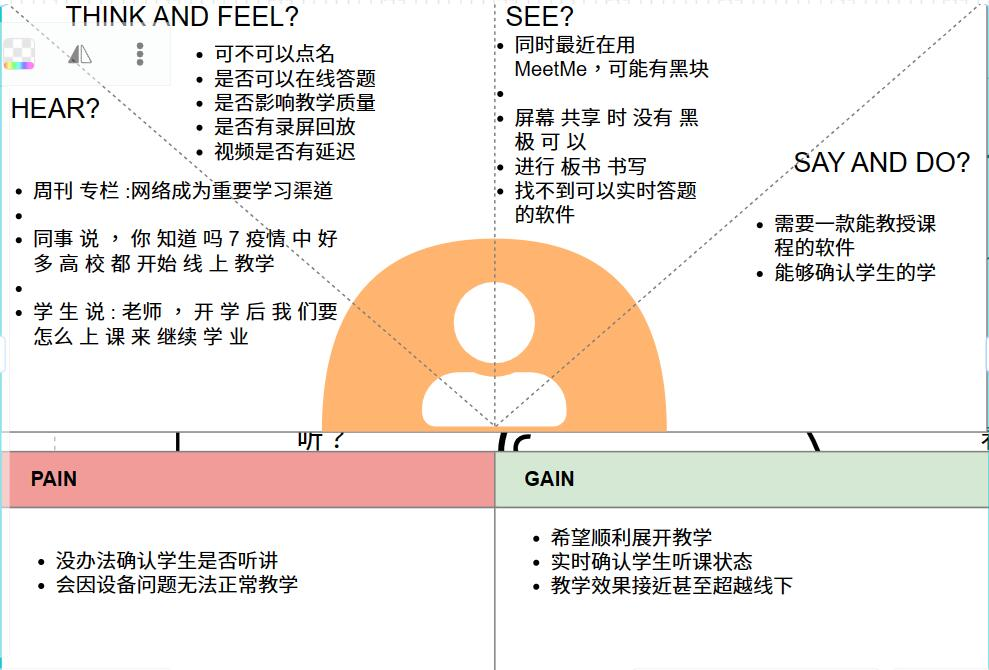
\includegraphics[width=0.8\textwidth]{高校移情图.jpg}
        \caption{Your caption}
    \end{figure}
    \clearpage


    \subsection{企业主管}
    在企业会议中,我们的软件支持多人共享屏幕和远程设备操作,并且能够将会议文件安全地保存在云端。对于重要的会议,特别是涉及商业机密和重要客户资料的高层级会议,我们提供了加密算法来保护数据传输安全,以防止黑客入侵和信息窃取。

    对于跨国企业的企业主管,我们的软件可以满足其与各国小组成员或支持业务部门进行安全交流与会议的需求。在跨国交流中,可能涉及公司的敏感信息和机密数据,因此我们提供了可靠且安全的软件来保障交流的安全性。

    通过我们的软件,企业主管可以放心进行跨国远程交流,而无需担心信息安全问题。我们致力于提供高质量、安全可靠的会议解决方案,以满足企业在全球范围内的远程会议需求。
    \begin{figure}[h]
        \centering
        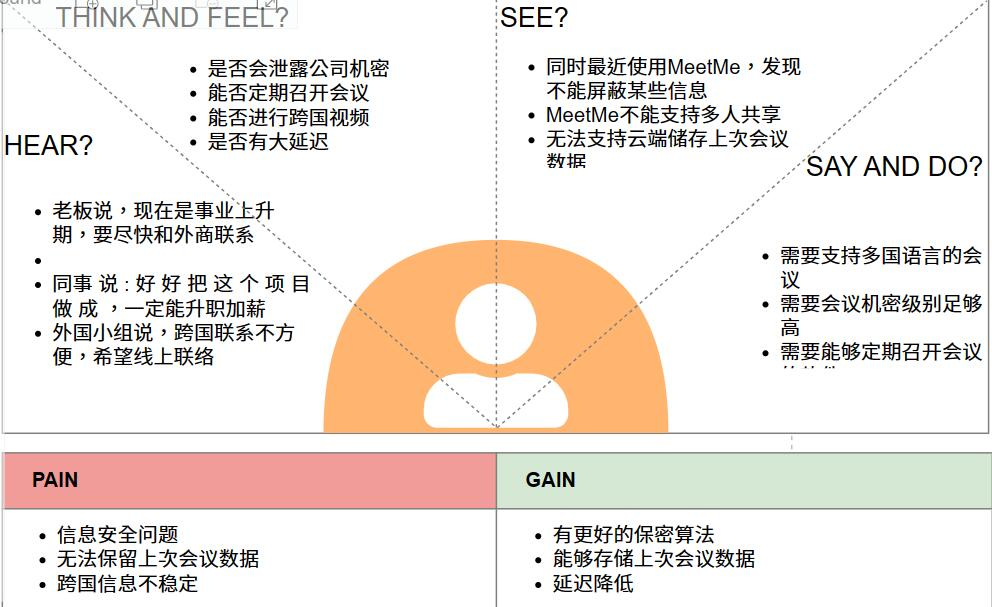
\includegraphics[width=0.8\textwidth]{企业移情图.jpg}
        \caption{Your caption}
    \end{figure}
    \clearpage


    \subsection{电影爱好者}
    本平台通过向大量的流媒体公司购买公开放映的版权,获得音乐和视频的播放权。我们在会议中添加了娱乐功能,让会议不再局限于严肃的教学和办公,而是为大家提供一个娱乐和放松的空间。在我们的会议平台上,与会者可以一起阅读书籍、共同观赏电影、共享音乐等。

    阿水是电影同好会的成员,他和他的社团成员因为地理位置不同,无法随时聚在一起。因此,他正在寻找一个便捷的方式,在周末与社团成员一起观影。我们的平台正是为了满足像阿水这样的用户需求,让他们能够通过我们的会议平台,轻松地一起观赏电影,即使身处不同的地理位置也能共享同样的娱乐体验。
    \begin{figure}[h]
        \centering
        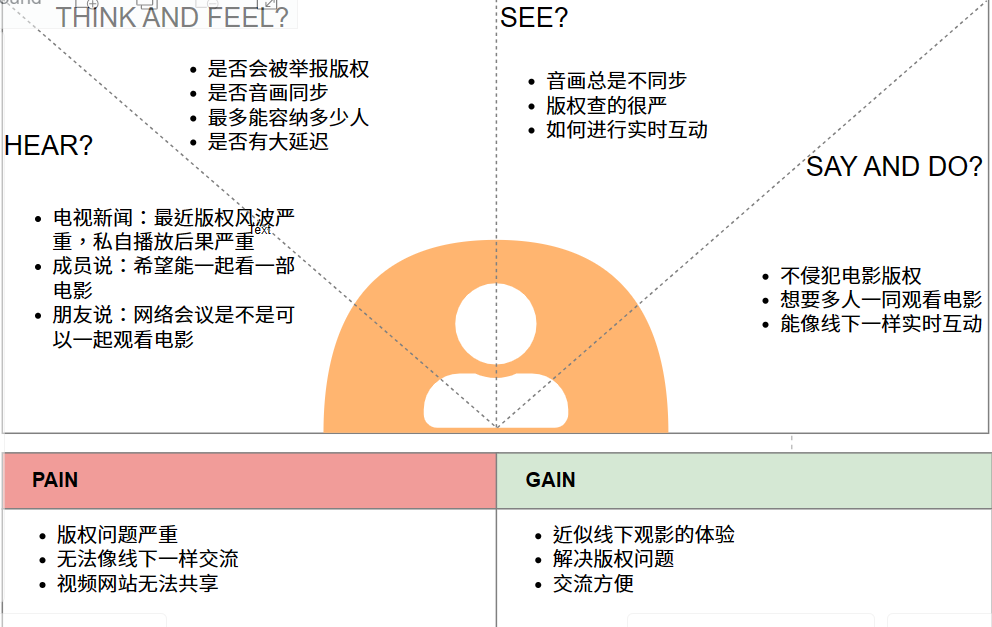
\includegraphics[width=0.8\textwidth]{电影爱好者移情图.png}
        \caption{Your caption}
    \end{figure}
    \clearpage

    \section{构思}
    \subsection{从财务驱动的角度出发}
    如果我们在产品上线的初期通过向云服务商购买云服务器资源的方式来缩减向用户提供云服务的成本会怎么样?

    自行进行云服务器的搭建这一项活动本身是重资产的,在产品上线的初期,我们可能是没有足够的资金来进行服务器的购置和云服务器的构建的。尽管有人会说,我们可以像ofo和瑞幸一样,只要饼画的足够的好,就能吸引足够的融资来实现重资产的想法。这样的想法是太过于幼稚的,要知道,我们自行构建云服务器的想法在营收上就不是太为乐观的,就算是可以像阿里一样将闲置的计算资源开发成提供阿里云的方式来带来营收,其回报率在短时间内是较低的,很容易就会像ofo一样在最后不堪重负,连押金都退不回来;除此之外,技术的限制才是最大的问题,高昂的开发成本和维护成本对我们这样刚开始运营的公司的压力是巨大的,很有可能就是适得其反的行为。因此,在我们产品上线的初期,我们更倾向于与云服务商合作,并向其购买云服务器资源来为我们的用户提供云服务的方式。这样的成本是相对可控并且较为低廉的,可以在初期尽可能的帮我们缩减成本,以维持我们更好的商务运营。

    \subsection{从客户驱动的角度出发}
    如果客户觉得我们的界面交互不够人性化,吐槽或提出建议会怎么样?

    首先,我们的产品是有一个用户可以向我们反馈问题的“社区”的,用户任何吐槽或者建议都可以通过“社区”或者问卷的形式向我们进行反馈。我们会对用户的反馈采用聚类的技术来进行共性问题的筛选。对于对我们人性化功能的建议在通过我们产品部门的调整和优化之后,会提交给技术部门实现,然后上线测试版本,同时再通过问卷的形式听取测试版本使用者的反馈,来进行取舍和再优化。对于一些可能是部分受众所青睐的交互方式,我们会设计成可选项,方便用户进行自定义,最终达到每个用户都能拥有最舒适的体验感,达到近乎于“私人订制”的境界。

    \subsection{从供给驱动和财务驱动的双重角度出发}
    如果我们产品对基础使用进行免费,为一些想要拥有更为个性化设置、更长会议时间、更多最大参会人数、更大的云存储空间等的用户提供收取一定费用的VIP服务会怎么样?

    针对不同的客户群体提供不同的服务,这是有利于我们吸引不同样的客户群体的。对于产品的基础使用提供免费的服务,而且基础的使用也能给客户较为舒适的使用体验,这在产品发行的前期是十分有利于我们口碑的积累的,拥有足够优秀的口碑可以帮助我们在这个赛道拥有自己的一席之地,从而拥有持续发展生存的基础。同时我们会提供一定的增值服务,为一些拥有对更为个性化设置、更长会议时间、更多最大参会人数、更大的云存储空间的需求的用户,我们会为其提供更多的资源,同时收取一定的服务费用,从而成为我们的一项收入来源,帮助我们更好的持续发展。

    \subsection{从客户驱动的角度出发}
    如果客户在使用过程中对指定的用户群有频繁会议连接的需求会怎么样?

    很多用户在使用过程中会对指定的用户群有频繁会议连接的需求。如果还需要通过其他渠道来分享会议链接,会给客户带来额外的工作量,很有可能会引起客户对”繁琐“流程的反感。因此,面对上述的问题,我们的产品会提供简洁且有针对性的社交系统,客户可以通过我们的社交系统建立自己的联络网、通讯录,然后就可以在我们的社交系统内直接“一键”向指定的用户分享会议邀请链接,指定用户就可在我们的社交网络中进行接受邀请或者拒绝邀请的操作,从而形成用户之间的“互联”,满足客户在使用过程中对指定的用户有频繁会议连接的需求,大幅降低客户之间交流的成本,提高工作的效率。

    \subsection{从资源供给的角度出发}
    如果我们的视频软件平台使用自己的云服务会怎么样?

    对于视频会议软件,云服务的可靠性和安全性的要求是非常高的。如果我们全部使用自己的云服务器进行服务,为了维持应用级容灾的成本会非常恐怖。所以我们倾向于将软件开发初期的云服务委托给外部的第三方服务商,使用它们已经成熟的技术对服务的稳定性进行保证。保证核心用户数据以及私人的隐私信息在我们自己的服务器集群中,在软件达到一定的规模之后可以使用自己的云服务进行一定的替换,对数据安全性能够提更高的保障。

    \subsection{从客户驱动角度出发}
    如果软件平台没有客户想要的影视作品,我们根据客户需求引入会怎么样?

    对于平台内缺少的影视作品,用户可以提出引进需求,每隔 1-2 周平台进行一次统计,对需求量最大的前几名予以引入。从客户关系角度出发,能够按用户的需求引入影片,无疑 会让我们留住更多的老客户,同时我们也会新增“按用户需求供给影片”的价值主张。这 种新颖的服务也有助于我们价值主张的传递,能够扩大我们的知名度。问题在于会加剧成 本结构中版权费的资金消耗,但是相应的影视资源的会员费用收入来源也会得到强化。我们的核心资源,重要合作,关键业务都 不会受到影响。还有一个问题是,如果客户需求的 影片我们无法获取,该如何避免用户失望的情况出现(我想到的办法是,早期征求需求的 时候,影片的需求数量排名不公平,直到成功引进 后,才公布引进的内容。)

    \subsection{从财务驱动的角度出发}
    如果我们放弃广告费和使用费的收入,专心去做会员费和许可使用费的收益最大化会怎么样?

    这种收入来源的变革分别有各自的原因,一是广告市场在谷歌、百度等巨头的压榨下,已 基本饱和,广告难有高额利润可寻,广告本身也成为用户反感的痛点;二是免费商业模 式的迷人之处就在于免费的商品会吸引数量庞大的客户。因此,我们计划制作一款“纯粹”的软件产品。无广告植 入和免费的功能使用无疑会带来广阔的客户群体。自然,这种免费不是无限制的免费,我们会在使用次数和功能选择上提供限制,即让偶尔使用我们产品的客户可以维系得住,因为他们随时可能变成经常使用的活跃客户;主要的收入则从活 跃客户里获取,我们会对会员进行服务进行精致化打 造——无限使用时间,扩充存储空间等等。这种财务驱动的创新并不会对我们的整体画布有巨大的 改变,但在客户细分这个要素上,这种方式会使得越来越多的边缘客户和潜在客户愿意了解我们, 并向我们付费。这里面体现的思路是——做“免费且纯粹好用”的软件是可以吸引海量客户的,而当 基数达到一定程度,其中选择支付费用获得更好服务的人也会随之越来越多。

    \subsection{从多点驱动的角度出发}
    如果我们给我们的视频以及影像资料提供双语甚至多语服务会怎么样?

    由于我们的最终目标是向国际化的方向进行发展,对我们的软件的国际化程度有较高的要求。在我 们增加了双语或者是多语的多种字幕和社交系统时,可以吸引不同的客户群体进入我们的软件进行 消费,同时可以更好的服务于跨国业务。当客户在软件中能够体验到跨国家跨语言的无障碍交流 时,自然就能对软件产生用户粘性。我们提供的翻译服务是由第三方的翻译供应商进行服务的。从 客户的角度看,即使客户是跨国跨语言的,但是还是能通过多语言的字母来实时观看展示的成果, 为客户减轻了一定的语言学习成
    \section{视觉化思考}
    \subsection{可视化讲述及花絮}
    \subsection{可视化画布}
    \subsubsection{价值主张}
    \subsubsection{客户细分}
    \subsubsection{关键业务}
    \subsubsection{渠道通路}
    \subsubsection{客户关系}
    \subsubsection{收入来源}
    \subsubsection{关键资源}
    \subsubsection{重要合作}
    \subsubsection{成本结构}
    \subsection{改进}
    \section{模型构建}
    \subsection{商业模式画布}
    \begin{figure}[h]
        \centering
        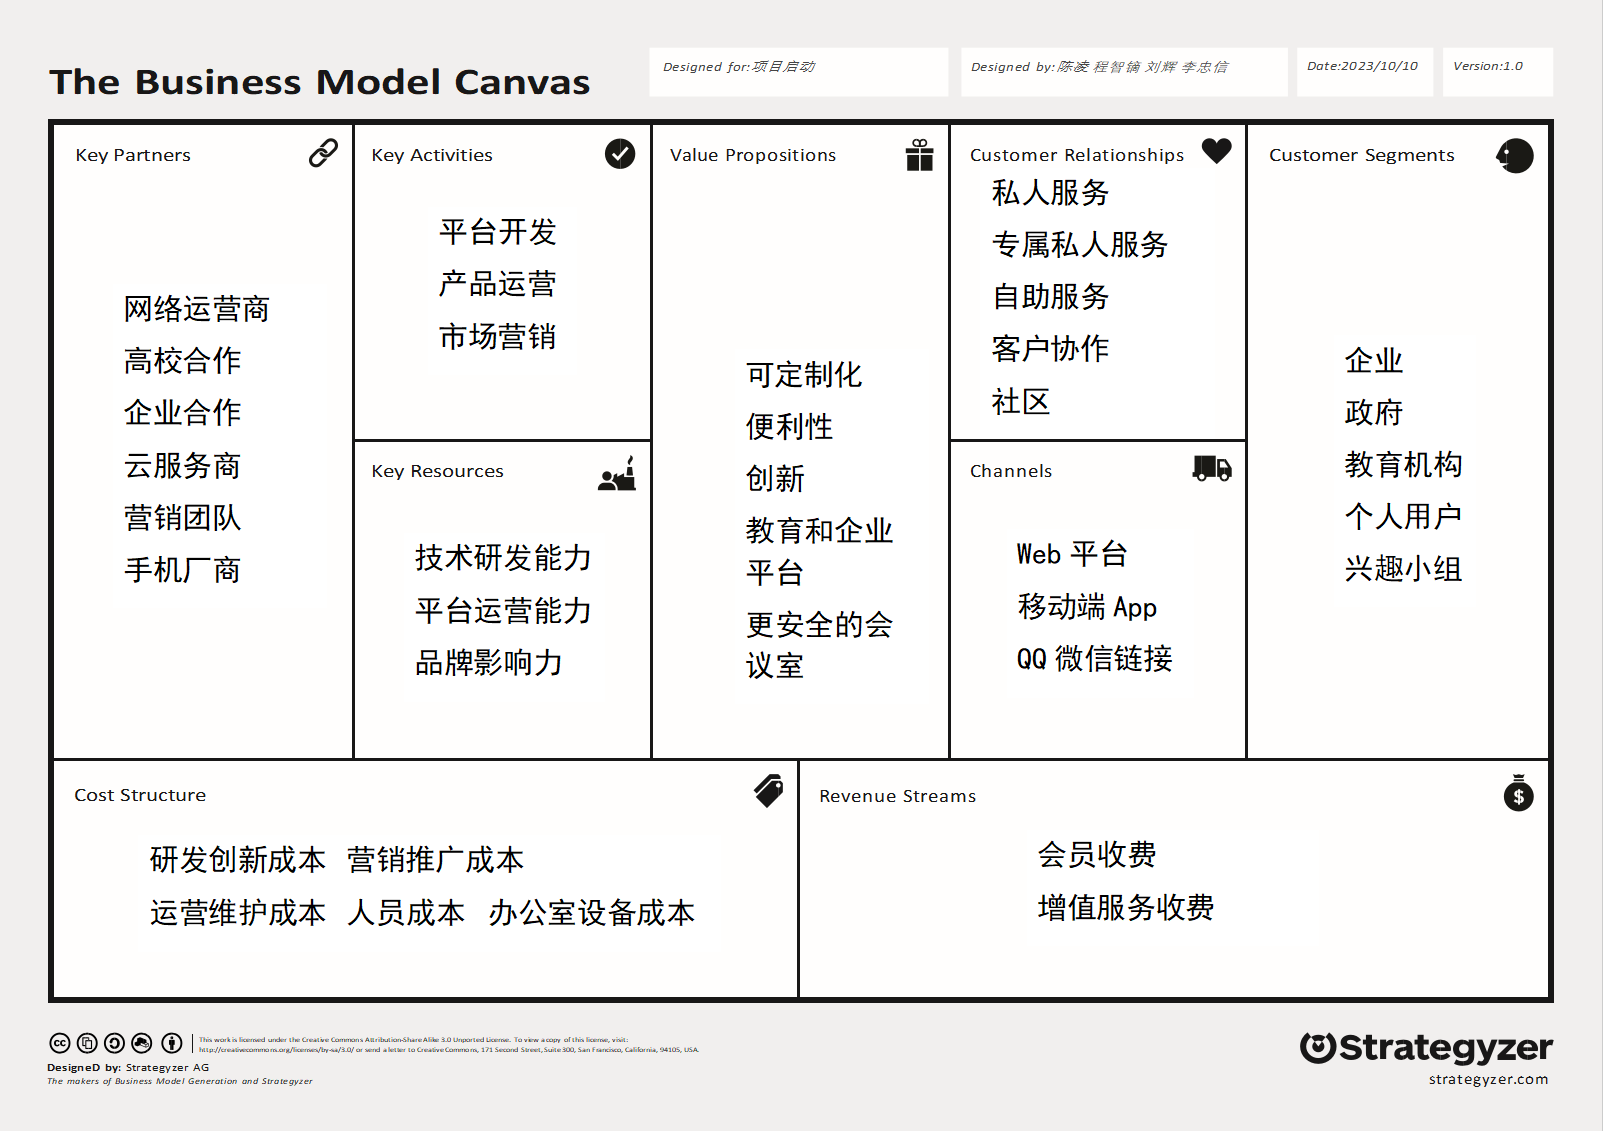
\includegraphics[width=0.8\textwidth]{第3次商业模式画布.png}
        \caption{商业模式画布}
    \end{figure}
    \clearpage
    \subsection{要点介绍}
    \subsubsection{关键业务}
    \noindent 普通会议:针对大多数普通用户的远程线上会议

    1.使用者可以建立临时会议或预定特定时间的会议,并邀请与会者入会。

    2.使用者可以将指定会议加入时间规划中,设置提醒时间。

    3.使用者可以添加联系人,并直接向联系人发送会议邀请。

    4.使用者可以在会议中选择开启视频功能或语音功能。

    5.使用者可以上传会议回放或文件至云端供所有与会者查看

    \noindent 教学会议:针对教学目的的远程线上会议,在普通会议的基础上增加为教学服务的功能,例如在线答题,讨论组等功能

    \noindent 企业会议:针对企业进行的远程线上会议,在普通会议的基础上增加为企业服务的功能,例如多人同时共享,多设备同时操作,会议加密等功能

    \noindent 娱乐会议:针对娱乐需要进行的远程线上会议,或者称之为派对,支持可联机进行的休闲活动例如一起观看电影综艺,一起听歌,彻底打破会议的传统模版

    \subsubsection{客户细分}
    1.想要临时召开线上会议的普通用户

    2.想要拥有更多个性化设置,更长会议时间,更多与会人数,更大云端存储空间,并愿意付费的VIP用户

    3.想要线上授课并以此谋利的教学机构

    4.想要进行线上会议办公的企业或政府

    5.想要进行远程联机娱乐的群体用户、兴趣小组
    \subsubsection{价值主张}
    1.可定制化:用户可以根据类型选择会议,会议也提供诸多可细分的可选选项设置,充分定制自己理想中的会议

    2.便利性:最大地简化用户的操作,例如,在已经收到邀请的情况下,用户不再需要输入会议号和密码即可进入会议,在已经设置了会议规划的情况下,可以直接从规划中点击进入会议。

    3.创新:打破原有会议软件功能单一的缺点,将会议类型化,对不同类型会议设置不同的功能与条件,不仅有普通的会议,还有针对教育,针对企业,针对娱乐目的的多功能化会议。在线上会议的基础上探索更多远程会议的根本功能和盈利方式,尽可能地模拟线下会议。

    4.教育和企业平台:产品最大限度地在线上满足教育与企业线下活动的条件。针对教学会议,设立线上答题功能,并由产品统计答题结果给会议主持者。针对企业会议,多人共享,讨论组等功能满足了成果展示,面试等基本企业活动所需的条件。

    5.更安全的会议室:产品为企业或者教育机构提供安全性更高的会议室
    \subsubsection{渠道通路}
    合作伙伴渠道(QQ,微信等):

    1. 知名度:

    1.1 可以通过与学校,教育机构,企业,个人(以公开会议盈利,有一定的知名度)的合作
    与宣传,提升自身知名度。

    1.2 同时教育机构,个人高品质的会议与成果会吸引更多的使用者使用该产品,或者促进其
    他机构与个人与产品的合作。

    1.3 会议是群体性行为,好的会议效果也会让使用者使用该产品的同时,推动群体其他成员
    使用该产品,通过社交裂变的方式不断扩大产品的使用群体。


    2. 购买:与企业、高校、教育机构合作,提供企业优惠、教育优惠等,高校和大企业等能够以
    优惠价格购得团体专属使用权。

    \noindent 自身渠道(Web平台):
    1. 知名度:制作官方网站,方便用户更好的了解我们,并且潜在用户在浏览到我们的网站时可以提
    高知名度。

    2. 评价:通过问卷、问题反馈、在线客服等反馈机制让用户对产品功能和价值主张进行评估。

    3. 购买:普通用户在我们制作的官方网站上或者软件内可以购买到VIP服务;企业、高校、教育
    机构等群体可以联系产品的团体使用负责人购买团体专属使用权。

    4. 传递:通过使用手册及操作引导的形式让用户明确产品的价值主张。

    5. 售后:有智能客服和在线人工客服,向客户提供售后支持。
    \subsubsection{客户关系}
    1.私人服务:有在线人工客服,与客户进行实时一对一交流,提供帮助

    2.专属私人服务:针对大企业,高校,有专门负责人维持合作关系,提供个性化定制服务

    3.自助服务:用户可以自行创建或参与会议,用户可以自行选择会议类型

    4.与客户协作,共同创造:教育机构可以通过会议向其他使用者开展课程,创造教育价值

    5.社区:提供在线社区平台,供客户交流使用心得,帮助彼此解决问题,也能帮助开发者更好地了解客户的需求,使我们的产品更加人性化
    \subsubsection{收入来源}
    1.会员费:对想要拥有更多个性化设置,更长会议时间,更多与会人数,更大云端存储空间,并愿意付费的VIP用户收取会员费

    2.增值服务使用费:对于一些有版权收费的娱乐项目对使用者收取相应费用或向教育机构和企业收取相应会议使用权的购买费用
    \subsubsection{核心资源}
    1. 技术研发能力:对于各种会议中视频需求所需要的流媒体的设备支持、对会议过程中的视频音频提供稳定的连接服务,防止卡顿或延迟

    2.平台运营能力

    3.品牌影响力:对于本软件的广告营销宣传的专业团队

    \subsubsection{重要合作}
    1. 运营商网络合作:对于会议过程中传输的流媒体数据需要运营商提供足够带宽来进行支撑。

    2. 高校合作:远程会议软件可以作为高校的线上课程的一个使用平台,与高校的合作可以促进高校师生之间的线上交流,同时推广软件。

    3. 企业合作:远程会议软件可以作为企业线上会议的一个适用平台,可以便于各地的子公司之间的联系。

    4. 云服务商:会议软件需要大量的云服务器作为平台支撑,通过与云服务商的合作可以将用户的数据同步到云端,保证数据的安全性,同时不必浪费用户本地的磁盘空间。

    5. 营销团队:软件和营销团队之间的合作能够让软件在大众中的知名度有所提升,能使软件成为个人用户远程会议的首选。

    6. 手机厂商:与手机厂商合作在手机里预安装软件以扩大软件的使用量和知名度
    \subsubsection{成本结构}
    1. 研发创新成本:软件在开发创新功能时所需要的成本。

    2. 运营维护成本:在软件开发初期,一般使用成型的云服务平台节省成本,扩大存储空间,需要支付云服务器的费用。

    3. 营销推销成本:在软件宣传的过程中,需要大量的广告宣传来提高知名度,巩固在大众之中的地位。

    4. 员工工资:软件在开发维护时所需要的开发维护人员的薪资。

    5. 办公室设备成本:软件发布之后需要有客服人员以及维护人员持续提供服务,需要一定的成本对职员的办公设备进行维护。

    \subsection{关联}
    1. 1.1.5 (云存储)、6.1 (增值服务使用费)为了使用户的会议记录可随时随地反复观看,我们为其提供一定量的云存储空间,如果用户需要更大的云存储需求,将对其进行按量收费

    2. 1.1.3(联系人) 、1.1.1(邀请入会) 为了用户之间的更好关联,我们加入了联系人系统,用户可以增加常用联系人,并可以向联系人直接发送邀请

    3. 1.1.2(会议规划)、3.2(便利性) 我们内置了日历工具,帮助用户规划日程安排

    4. 1.2 (教学会议)、2.3 (教学机构) 5.4 (用户协作)为教育机构专门打造的教育会议,共同创造教育价值

    5. 1.3(企业会议)、2.4(企业用户)为企业打造的企业会议,创造面对面开会的氛围

    6. 1.5(娱乐会议)、2.5(娱乐用户)、6.3(增值服务使用费)用户创建娱乐会议,自助服务进行娱乐资源的选择。产品和流媒体平台合作,进行资源的共享,提供给用户高质量的娱乐资源,同时支付流媒体平台视频版权费用,向用户收取娱乐资源使用费用

    7. 2.2(VIP用户)、3.1(可定制化)、6.1(会员费)为一部分想要拥有更多功能并愿意付费的用户提供的VIP服务,可以通过官方渠道开通,为我们带来收益

    8. 3.3(创新)、1.2(教学会议)、1.3(企业会议)、1.4(娱乐会议) 产品在普通会议上进行创新,提供不同场景的不同会议模式。

    10. 3.6(教育和企业平台)、1.2(教学会议)、1.3(企业会议)通过充分模拟教学与企业所需的条件,给予用户可靠的平台体验

    11. 4.1.1.1和4.1.1.2(合作与宣传)、8.2(高校合作)、8.3(企业合作)通过与高校与企业合作与宣传,提升自身知名度

    12. 4.2.2(评价)、5.5(社区)用户可以通过反馈机制和社区等形式,对我们的业务做出评价,提出想法,我们采纳合理的评价

    13. 4.2.5(售后)、5.1(私人服务)、9.1(员工成本)、9.4(办公室设备成本)用户可以通过客服的私人服务,对我们的产品进行售后,为此公司需要支付员工工资和办公室设备采购和维护

    14. 5.2(专属私人服务)、2.3(教育机构)、2.4(企业用户)、4.1.2(合作伙伴渠道购买)、4.2.3(自身渠道购买) 企业、高校等群体可以通过专属的私人服务联系产品负责人。

    15. 7.2(平台运营能力)、8.4(云服务商)、9.2(运营维护成本)与云服务商深度合作,使用成型的云服务平台,为此需要支持云服务器使用费

    16. 7.2(平台运营能力)、8.1(运营商合作)对于会议过程的视频和音频传输需要稳定的运营商提供的带宽支撑

    17. 8.5(营销团队合作)、9.3(营销推销成本)与营销团队进行合作,通过营销宣传扩大产品影响力,将此作为产品的宣传资源,为此需要支付一定的广告费用
    \subsection{基本事实与分析}
    \textit{近年来,视频会议供应商不断更新硬件和软件,从依赖使用专用解码、传输等设备的传统视频会
    议,发展到基于互联网的软件视频会议,目前已出现了具有云功能的视频会议设备、收集大数据
    以获得更个性化服务的分析软件。
    从视频会议的应用领域及应用场景来看,视频会议可应用于医疗、教育、金融等领域,应用场景
    主要包括商务谈判、销售会议、任务部署和工作协调、工作汇报及例会等。
    从视频会议的产业链来看,视频会议产业链的上游主要为芯片及元件提供商和视频解码技术等提
    供商,产业链中游主要为视频会议系统及解决方案的提供商,下游为集成商、代理商以及视频会
    议的用户。}\footnote{前瞻产品研究院}

    \textit{伦敦大学亚非学院博士在读的薛同学表示,线上授课本身是科技发展的一个重要产物,甚至
    并不是一个短期性、阶段性的产物:“今后社会发展肯定会在各个维度、各个层面采用线上交流的
    形式,因此,作为年轻人主动适应新形势的变化也必须的。”
    据薛同学介绍,从3月初开始,大多数英国高校就开始让学生自己选择是否愿意返校上课。疫
    情刚开始的前几周,学校采取线上辅导讲座、线下教室讲授课程内容的形式。在3月底以后学校就
    采用了全网课的形式直至现在。根据学校的要求,目前全年度都采用线上的形式,同时,学生可
    以暂时选择不前往英国进行入学注册,可以选择在各自的国家进行线上听课。学校也有相对的应
    急措施,包括提供全时段的学术交流平台、帮助录课、虚拟授课论坛等,这些形式最近也是大多
    数学校所选择的方式。}\footnote{中国侨网}

    这些新闻都证实了疫情期间大量的视频会议软件的需求出现在市场上,疫情过后这个需求并没有出现显
    著的跌落,还是有一定的增长势头。同时由于现阶段信息安全的问题日益凸显,软件必须专注于自己的
    加密技术。分析现有的视频会议软件即可发现,现在市场上的会议软件基本上专注于进行视频会议的工
    作,对应因为COVID-19猛增的工作会议和教学会议需求,同时对不同的会议种类并没有做精细的分
    类。在使用市场中已经存在的视频软件的时候经常会出现会议要求某种功能但是不存在的情况,同时会
    出现在目的性较强的会议中出现不需要的冗余功能导致会议的流畅度受到影响。

    我们的软件致力于对具有目的性的会议提供更加专业的软件服务环境,在企业用户使用时我们为企业用
    户提供专业级的企业视频会议的服务模式,能够对企业级的会议中经常需要的功能进行实现,对企业的
    会议进行专项的优化。在针对教育机构或是学校的会议中,我们提供完整的签到和一定的答题功能,能
    够让老师在上课的过程中对学生的集中程度和对课程的反应程度进行一定的评估。针对多种不同的会议
    模式提供各种不同的功能,能够让用户拥有更加好的服务体验。

    \textit{整体上,以Zoom Meeting为基础,其余产品类似于Zoom Rooms、 Zoom Phone 、Zoom
    Video Webinars 都是在此基础上的功能的延伸与拓展。
    基于上述产品,它们会针对医疗、教育、政府及金融领域,并推出相应产品满足行业定制化需
    求。
    从商业模式看来,Zoom以「Free+Prime」——也就是免费增值模式切入市场,对不同用户采用
    差异化定价。
    对于一般用户而言,允许免费使用,但是限制会议时间、参与人数等功能。订阅用户能够使用的
    功能更多,也更加完善。}
    \footnote{知乎(量子位)}

    从上述的分析报告中可知市面上的视频软件的数据显示服务器的支付费用是视频软件的一项重要费用。
    同时市面上的视频软件比较常用的的收入手段就是广告推广费用,这也将成为我们的MeetMe软件的重要
    收入来源。我们的软件致力于使用用户对软件的依赖性,吸引用户进行支付升级会员作为我们的收入来
    源,我们将为用户提供一定量的免费存储空间,为用户的会议提供历史存储,但是当用户需要更多的存
    储空间对历史的会议进行存储时就需要支付额外的费用,同时用户使用娱乐板块的有版权的内容时也需
    要支付对应的版权费用。用户也可以直接选择平台的会员费用,在一次性进行了支付之后,会员时间内
    产生的额外费用将由平台进行承担。我们也期望通过适量的广告进行流量引流的宣传费用。
    \subsection{市场潜力预估}
    MeetMe的软件优势在于我们将严肃的视频会议软件和现阶段最流行的视频和流媒体软件进行融合,我们希望吸引需要使用视频会议软件的企业以及教育机构的用户同时使用MeetMe软件进行一定的娱乐。由于现在这两个方面都已经有成型的软件,所以需要用户对我们的软件产生较为满意的使用体验是相对
    困难的。我们希望通过我们边界的一站式服务的用户体验来吸引用户进入平台,同时通过精准的推荐系统和精简的界面让用户认同我们的软件产品。随着网络通信技术的不断革新导致现在出现了更多的人与人之间需要沟通介质的情况出现,传统的语音视频通话难以向对方展示内容,而现有的视频会议软件针对各种会议的精准服务的能力较差,我们希望吸引需要视频会议软件的有高准确度的目标定位的用户进入我们的软件进行消费,成为我们软件的最佳用户。结合我们软件的一站式服务体验,我们认为我们的软件是具备较强的市场发展潜力的。
    \section{讲故事}
    \section{场景}

\end{document}
